\documentclass[10pt]{article}
\usepackage[a4paper, margin=0cm]{geometry} 
\usepackage[utf8]{inputenc}
\usepackage[T1]{fontenc}
\usepackage[sfdefault]{roboto} 
\usepackage{fontawesome5} 
\usepackage{graphicx} 

% --- 核心设置 ---
\usepackage{tikz} 
\usetikzlibrary{positioning, arrows.meta, shapes, calc, backgrounds, shadows} 
\usepackage{tcolorbox}
\tcbuselibrary{skins, raster, fitting}

% --- 颜色定义 ---
\definecolor{DarkNavy}{HTML}{0A244D} 
\definecolor{TechCyan}{HTML}{00F0FF} 
\definecolor{AccentBlue}{HTML}{3A86FF}   
\definecolor{LightBlueBg}{HTML}{E6F4FF}  
\definecolor{SoftRedBg}{HTML}{FFF0F0}
\definecolor{LightGreenBg}{HTML}{E8F5E9} 
\definecolor{RedText}{HTML}{D90429}      
\definecolor{TealText}{HTML}{008080}
\definecolor{GreenText}{HTML}{2A9D8F}    
\definecolor{SectionTitle}{HTML}{2B2D42} 
\definecolor{CardBorder}{HTML}{E0E0E0} 

% --- 全局排版 ---
\pagestyle{empty}
\setlength{\parindent}{0pt}
\setlength{\parskip}{0pt}

% --- 自定义样式 ---
\newtcolorbox{headerbox}{
    enhanced, colback=DarkNavy, colframe=DarkNavy, sharp corners, boxrule=0pt,
    width=\paperwidth, 
    top=0.3cm, bottom=0.3cm, left=1.5cm, right=1.5cm,
    colupper=white, valign=center
}

\newtcolorbox{contentbox}[2][]{
    enhanced, title={\large \textbf{#2}},
    colback=white, colframe=CardBorder, coltitle=SectionTitle,
    attach boxed title to top left={xshift=4mm, yshift=-3mm},
    boxed title style={colback=white, frame hidden},
    fonttitle=\large\bfseries,
    boxrule=1pt, drop shadow,
    top=1mm, bottom=1mm, left=2mm, right=2mm,
    nobeforeafter,
    arc=3mm,
    #1
}

\newtcolorbox{resultbox}[2][]{
    enhanced, title={\large \textbf{#2}},
    colback=white, colframe=AccentBlue!40, coltitle=SectionTitle,
    attach boxed title to top left={xshift=4mm, yshift=-3mm},
    boxed title style={colback=white, frame hidden},
    fonttitle=\large\bfseries,
    boxrule=1.5pt, drop shadow,
    top=1mm, bottom=1mm, left=2mm, right=2mm,
    nobeforeafter,
    arc=3mm,
    #1
}

\newtcolorbox{alertbox}[2][]{
    enhanced, colback=#2, colframe=#2, leftrule=3mm,
    colframe=gray!20, borderline west={3pt}{0pt}{#2!60!black},
    arc=2mm, boxrule=0pt, top=1mm, bottom=1mm, fontupper=\small,
    #1
}

\newtcolorbox{conclusionbox}[2][]{
    enhanced, title={\large \textbf{#2}},
    colback=DarkNavy, colframe=DarkNavy, coltitle=white,
    attach boxed title to top left={xshift=4mm, yshift=-3mm},
    boxed title style={colback=DarkNavy, frame hidden},
    fonttitle=\large\bfseries, colupper=white,
    drop shadow, arc=3mm,
    top=2mm, bottom=2mm, left=2mm, right=2mm,
    #1
}

\begin{document}

% =========================================
% 1. HEADER
% =========================================
\begin{headerbox}
    \begin{tikzpicture}[remember picture, overlay]
        \node[absolute, anchor=north east, opacity=0.08, xshift=-1cm, yshift=-0.5cm] at (current bounding box.north east) {
            \begin{tikzpicture}
                \draw[white, line width=2pt] (0,0) circle (2cm);
                \draw[white, line width=1pt, dashed] (0,0) circle (2.8cm);
                \node[text=white, font=\bfseries\huge] at (0,0) {\faAtom};
            \end{tikzpicture}
        };
        \fill[white, opacity=0.03] (current bounding box.south west) -- ++(4,4) -- ++(8,0) -- (current bounding box.south east) -- cycle;
    \end{tikzpicture}

    
\begin{tikzpicture}[baseline]
        \node[fill=TechCyan, text=DarkNavy, font=\bfseries\footnotesize, rounded corners=1pt, inner sep=3pt, anchor=base] (tag) {INTERIM PROGRESS REPORT};
        \node[right=0.3cm of tag, text=gray!60, font=\scriptsize, anchor=west] {INFORMATION RETRIEVAL SYSTEM DESIGN \ \textbullet\ \ \today};
    \end{tikzpicture}
    
    \vspace{0.15cm}
    {\fontsize{24}{28}\selectfont \textbf{Scalable Neural Search:\\[0.1em] Architecture Design \& Evaluation}}
    \vspace{0.15cm}
    {\color{gray!40}\hrule height 0.5pt}
    \vspace{0.15cm}
    
    \begin{minipage}{0.65\textwidth}
        \large \textbf{Haonan Zhang} 
        \par \vspace{0.1cm}
        \small \textcolor{TechCyan}{\faUniversity} \ School of Advanced Technology, XJTLU
    \end{minipage}%
    \hfill
    \begin{minipage}{0.30\textwidth}
        \flushright \scriptsize 
        \textcolor{gray!80}{\textbf{Keywords:}}\\[0.1em] 
        \textcolor{gray!60}{Neural Search, LTR, LambdaMART}
    \end{minipage}
\end{headerbox}

% =========================================
% 2. ABSTRACT
% =========================================
\vspace{-0.2cm}
\begin{center}
\begin{minipage}{0.96\paperwidth}
    \begin{contentbox}{ABSTRACT}
        \small
        This ongoing project addresses the efficiency bottleneck in deploying neural ranking models. We propose a \textbf{Multi-Stage Hybrid Architecture} that integrates lightweight Learning to Rank (LTR) with selective Neural Re-ranking. Preliminary results on MS MARCO demonstrate that our prototype achieves \textbf{99\% of Cross-Encoder accuracy} while delivering a \textbf{10x speedup} in retrieval latency (<100ms).
    \end{contentbox}
\end{minipage}
\end{center}
% =========================================
% 3. MAIN BODY
% =========================================
\vspace{-0.3cm}
\begin{center}
    \noindent
    \begin{minipage}[t]{0.96\paperwidth}
        \vspace{0pt}
        
        % --- LEFT COLUMN (40% Width) ---
        \begin{minipage}[t]{0.4\linewidth}
            \vspace{0pt}
            
            % [1] INTRODUCTION
            \begin{contentbox}{1. INTRODUCTION}
                \small 
                Current search systems face a dilemma: \textbf{Precision vs. Efficiency}.
                \vspace{0.05cm}
                \begin{itemize}
                    \setlength\itemsep{0pt}
                    \item \textbf{Neural Models (BERT):} Achieve SOTA relevance but incur high latency ($>500$ms/query).
                    \item \textbf{Lexical Models (BM25):} Extremely fast but fail to capture semantic nuances.
                \end{itemize}
                \vspace{0.05cm}
                \begin{alertbox}{LightBlueBg}
                    \textbf{\textcolor{AccentBlue}{Research Objective:}} To \textbf{develop and assess} a scalable hybrid framework that bridges the gap between \textbf{Neural Precision} and \textbf{System Efficiency}.
                \end{alertbox}
            \end{contentbox}
            
            \vspace{1.2cm}
            
            % [2] METHODOLOGY
            \begin{contentbox}{2. METHODOLOGY} 
                \centering
                \vspace{0.2cm}
                \begin{tikzpicture}[
                    node distance=0.5cm and 0.6cm,
                    auto,
                    scale=0.82, transform shape,
                    >=Latex,
                    thick,
                    mainbox/.style={
                        rectangle, rounded corners=4pt, 
                        minimum width=3.2cm, minimum height=1.0cm,
                        align=center, font=\footnotesize\sffamily\bfseries,
                        drop shadow={opacity=0.15},
                        draw=gray!30, line width=0.8pt
                    },
                    subbox/.style={
                        rectangle, rounded corners=2pt,
                        minimum width=2.0cm, minimum height=0.7cm,
                        align=center, font=\scriptsize\sffamily,
                        draw=gray!40, dashed
                    },
                    dataflow/.style={->, color=DarkNavy, line width=1.2pt},
                    featureflow/.style={->, color=orange!70, line width=1.0pt, dashed}
                ]
                    \node[mainbox, fill=yellow!10] (query) {\faSearch \ \ User Query};
                    \node[mainbox, fill=blue!5, below=0.6cm of query, minimum width=4.0cm] (stage1) {
                        \textbf{Stage 1: Retrieval}\\
                        \scriptsize \faDatabase \ Elasticsearch (BM25)
                    };
                    \node[mainbox, fill=cyan!5, below=0.6cm of stage1, minimum width=3.2cm] (stage2) {
                        \textbf{Stage 2: LTR Ranking}\\
                        \scriptsize \faCogs \ LambdaMART (LightGBM)
                    };
                    \node[mainbox, fill=green!5, below=0.6cm of stage2, minimum width=2.4cm] (stage3) {
                        \textbf{Stage 3: Hybrid Rerank}\\
                        \scriptsize \faBrain \ Cross-Encoder (Top-K)
                    };
                    \node[mainbox, fill=orange!10, below=0.6cm of stage3, minimum width=2.0cm] (result) {\faListOl \ \ Final Results};
                    \node[subbox, left=1.2cm of stage2, fill=gray!5, align=center] (features) {
                        \textbf{Feature Store}\\
                        \tiny (Offline Vectors)
                    };
                    \draw[dataflow] (query) -- (stage1);
                    \draw[dataflow] (stage1) -- node[right, font=\tiny, color=gray] {Candidates ($N=50$)} (stage2);
                    \draw[dataflow] (stage2) -- node[right, font=\tiny, color=gray] {Top-K ($K=10$)} (stage3);
                    \draw[dataflow] (stage3) -- (result);
                    \draw[featureflow] (query.west) -| node[above right, font=\tiny, pos=0.8, color=orange] {Query Emb.} (features.north);
                    \draw[featureflow] (features.east) -- node[above, font=\tiny, color=orange] {Dense Feats} (stage2.west);
                    \begin{scope}[on background layer]
                        \fill[gray!5, rounded corners] 
                            ($(stage1.north west)+(-0.2,0.2)$) -- ($(stage1.north east)+(0.2,0.2)$) -- 
                            ($(stage3.south east)+(0.2,-0.2)$) -- ($(stage3.south west)+(-0.2,-0.2)$) -- cycle;
                    \end{scope}
                \end{tikzpicture}
                
                \vspace{0.4cm}
                \raggedright \small
                
                \textbf{2.1. Multi-Stage Pipeline}
                \begin{itemize}
                    \setlength\itemsep{0.2em} \footnotesize
                    \item \textbf{Stage 1 (Recall):} Efficiently retrieve top-50 candidates using inverted indices (BM25).
                    \item \textbf{Stage 2 (Precision):} Re-rank using \textbf{LightGBM LambdaMART}. Features include lexical scores, statistical signals, and \textbf{pre-computed semantic vectors}.
                    \item \textbf{Stage 3 (Refinement):} Apply heavy Cross-Encoder only to the \textbf{Top-10} results for final polish.
                \end{itemize}
                
                \vspace{0.3cm} 
                \textbf{2.2. Key Optimizations} 
                \begin{itemize}
                    \setlength\itemsep{0.2em} \footnotesize
                    \item \textbf{Knowledge Distillation:} The LTR model is trained on soft labels generated by a teacher Cross-Encoder, learning to mimic neural ranking behavior.
                    \item \textbf{Vector Precomputation:} Document embeddings are computed offline, reducing online cost to simple vector lookups.
                \end{itemize}
                \vspace{0.2cm}
            \end{contentbox}
        \end{minipage}%
        \hfill
        % --- RIGHT COLUMN ---
        \begin{minipage}[t]{0.58\linewidth}
            \vspace{0pt}
            \begin{resultbox}{3. PRELIMINARY RESULTS} 
                \centering
                
                % === Row 1: Trade-off & Latency ===
                \begin{minipage}[t]{0.48\linewidth}
                    \centering
                    \textbf{\footnotesize 3.1. Accuracy vs. Latency Trade-off}\\[0.1em]
                    \includegraphics[width=\linewidth, height=3.0cm, keepaspectratio]{images/tradeoff_plot.png}
                    \par \raggedright \scriptsize 
                    \vspace{0.05cm}
                    \textbf{Discussion:} The scatter plot reveals a clear Pareto frontier. \textbf{LTR (Blue)} and \textbf{Hybrid (Green)} strategies occupy the optimal "sweet spot" (top-left).
                \end{minipage}
                \hfill
                \begin{minipage}[t]{0.48\linewidth}
                    \centering
                    \textbf{\footnotesize 3.2. Latency Breakdown (Online)}\\[0.1em]
                    \includegraphics[width=\linewidth, height=3.0cm, keepaspectratio]{images/latency_stacked.png}
                    \par \raggedright \scriptsize 
                    \vspace{0.05cm}
                    \textbf{Discussion:} Cross-Encoder latency is dominated by inference (green bar). LTR shifts this cost to feature extraction (orange bar), which is computationally cheaper and highly parallelizable on CPUs.
                \end{minipage}
                
                \vspace{0.3cm}
                {\color{gray!30}\hrule} 
                \vspace{0.3cm}
                
                % === Row 2: Offline Quality ===
                \begin{minipage}[t]{0.98\linewidth}
                    \centering
                    \textbf{\small 3.3. Preliminary Relevance Evaluation (NDCG@10, MRR)}\\[0.1em]
                    \includegraphics[width=0.9\linewidth, height=3.5cm, keepaspectratio]{images/offline_eval_comparison.png}
                    \par \raggedright \small 
                    \vspace{0.05cm}
                    \textbf{Initial Analysis:}
                    \begin{itemize}
                        \setlength\itemsep{0pt} \footnotesize
                        \item \textbf{LTR Performance:} Achieves an NDCG@10 of \textbf{0.99}. This proves that dense features + tree models can approximate deep learning relevance.
                        \item \textbf{Hybrid Strategy:} Further improves MRR and Precision@10, ensuring the very first result is highly relevant.
                        \item \textbf{Baseline Gap:} BM25 significantly lags behind (NDCG $\approx$ 0.75), highlighting the necessity of semantic re-ranking.
                    \end{itemize}
                \end{minipage}
                
                \vspace{0.2cm}
                
                \begin{minipage}[c]{0.98\linewidth}
                    \begin{minipage}[c]{0.40\linewidth}
                        \textbf{\small 3.4. Feature Importance Analysis}
                        \par \vspace{0.1cm}
                        \raggedright \small
                        Our initial ablation study suggests that \textbf{Dense Vectors} are the primary driver of quality (\textbf{60\%}), capturing semantic intent. \textbf{BM25 scores} remain essential (\textbf{30\%}) for exact keyword matching, preventing "semantic drift." Simple statistical features (\textbf{10\%}) provide a cheap robustness boost.
                    \end{minipage}%
                    \hfill
                    \begin{minipage}[c]{0.6\linewidth}
                        \centering
                        \includegraphics[width=\linewidth, height=4.0cm, keepaspectratio]{images/feature_importance.png}
                    \end{minipage}
                \end{minipage}
                
                \vspace{0.2cm}
                
                \begin{tcolorbox}[colback=LightGreenBg, boxrule=0pt, frame hidden, arc=2mm, left=3mm, right=3mm, top=1mm, bottom=1mm]
                    \centering \small
                    \textcolor{GreenText}{\faLightbulb\ \textbf{Key Architectural Insight}}
                    \par \raggedright \footnotesize \vspace{0.05cm}
                    The bottleneck in Neural Search is not model size, but \textbf{inference frequency}. By using LTR as a high-precision filter, we reduce the number of heavy inference calls from $N=50$ to $K=10$, ensuring predictable \textbf{P99 tail latency} suitable for production SLAs.
                \end{tcolorbox}
    
            \end{resultbox}
        \end{minipage}
        
    \end{minipage}
\end{center}

% =========================================
% 4. CONCLUSION (Full Width)
% =========================================
\vspace{-0.2cm}
\begin{center}
\begin{minipage}{0.96\paperwidth}
    \begin{conclusionbox}{4. PROGRESS SUMMARY \& FUTURE WORK}
        \begin{minipage}[c]{0.58\textwidth}
            \small \raggedright
            \begin{itemize}
                \setlength\itemsep{0.2em}
                \item[\textcolor{TechCyan}{\faCheckCircle}] \textbf{Current Status:} Engineered a scalable, high-throughput neural search architecture.
                \item[\textcolor{TechCyan}{\faCheckCircle}] \textbf{Preliminary Metrics:} Achieved \textbf{\textcolor{TechCyan}{99\% accuracy}} of BERT with \textbf{\textcolor{TechCyan}{10x speedup}} in retrieval latency.
                \item[\textcolor{TechCyan}{\faCheckCircle}] \textbf{Key Finding:} Initial tests suggest that \textbf{dense feature engineering + LambdaMART} is a viable alternative.
            \end{itemize}
        \end{minipage}%
        \hfill
        \begin{minipage}[c]{0.38\textwidth}
            \begin{tcolorbox}[
                enhanced,
                title={\small \faRocket \ \textbf{Next Steps Plan}},
                colback=white!5!DarkNavy, 
                colframe=TechCyan!30!DarkNavy,
                coltitle=TechCyan,
                colupper=white!95!gray,
                boxrule=0.8pt, arc=2mm,
                left=1mm, right=1mm, top=2mm, bottom=2mm,
            ]
                \raggedright \footnotesize
                \begin{itemize}
                    \setlength\itemsep{0.1em}
                    \item[\textcolor{TechCyan}{\faArrowRight}] \textbf{Dynamic Routing:} Query-dependent model selection.
                    \item[\textcolor{TechCyan}{\faArrowRight}] \textbf{User Study:} Collecting user data and questionnaires for further optimization.
                \end{itemize}
            \end{tcolorbox}
        \end{minipage}
    \end{conclusionbox}
\end{minipage}
\end{center}

\end{document}
